 \documentclass[conference]{IEEEtran}
\IEEEoverridecommandlockouts
%\usepackage{hyphenat}
\usepackage[ruled,vlined]{algorithm2e}
\usepackage{amsmath}
\usepackage{xspace}
\usepackage[binary-units=true]{siunitx}
\usepackage{ulem}
%\usepackage{censor}
\usepackage[table]{xcolor}
\usepackage{graphicx}
\usepackage{hyperref}
\usepackage{tabularx}

\usepackage{subcaption}
\usepackage{booktabs}
\usepackage{multirow}
\usepackage{listings}
\usepackage{dingbat}
\usepackage{mathtools}

\hypersetup{
    colorlinks=true,
    linkcolor=black,
    citecolor=blue,
    filecolor=black,
    urlcolor=blue}

\def\BibTeX{{\rm B\kern-.05em{\sc i\kern-.025em b}\kern-.08em
    T\kern-.1667em\lower.7ex\hbox{E}\kern-.125emX}}


\makeatletter
  \def\footnoterule{\kern-3\p@
  \hrule \@width 2in \kern 2.6\p@} % the \hrule is .4pt high
\makeatother


\begin{document}

\newcommand{\fslspm}{FSL-SPM\xspace}
\newcommand{\fslafni}{FSL-AFNI\xspace}
\newcommand{\afnispm}{AFNI-SPM\xspace}
\newcommand{\tristan}[1]{\color{orange}\textbf{From Tristan:} #1\color{black}\xspace}
\newcommand{\ali}[2]{\color{green}\textbf{Ali:} #1\color{black}\xspace}
\newcommand{\discuss}[1]{\uwave{#1}}


\title{Software variability in fMRI analysis:\\ comparing between-tool and numerical errors}

\author{Ali Salari$^1$, Other Authors$^1$, Tristan Glatard$^1$ \\
$^1$ Department of Computer-Science and Software Engineering, Concordia University, Montreal, Canada}

\maketitle
\begin{abstract}

Numerical and software variability broadly affect structural, diffusion, and functional MRI analyses. Numerical
variability originates in software updates or code
parallelization, whereas software variability reflects discrepancies between
models implemented in different analysis software packages. While numerical
and software variability were both shown to impact analysis outcomes, the
extent to which these sources of variability compare for a given
analysis remains understudied. This work presents a comparison of
numerical and software variability for group-level and subject-level functional MRI analyses.
We reproduced a previous comparison between functional MRI analysis
software packages FSL, AFNI, and SPM, which we extended to measure
numerical variability through Monte-Carlo arithmetic.
Although We found that between-tool variability was larger than numerical variability,
we identified brain regions that numerical perturbations simulated between-tool variability.
Furthermore, we found more numerical instability in thresholded maps than unthresholded ones
and individual analysis than group-level analysis results. \tristan{Abstract to be fixed}

\end{abstract}

\begin{IEEEkeywords}
  Numerical Instability, Reproducibility, Monte-Carlo arithmetic, Neuroimaging
\end{IEEEkeywords}


\section{Introduction}

Software variability has been highlighted as an important source of error
in fMRI analysis, originating from mainly two factors: Between-tool
variability denotes differences observed in results produced by different
software toolboxes --- such as FSL, AFNI and SPM --- when analyzing the same dataset
using similar methods. Numerical variability, in contrast, denotes
differences observed in results produced by the same analytical toolbox
executed in different environments – such as different operating systems or
different hardware platforms. This manuscript investigates the extent to
which both types of variability relate to each other.

Numerical variability stems from errors introduced in floating point
computations by numerical rounding, cancellation and absorption~\cite{muller2018handbook}. In
practice, the occurrence of such errors is affected by variations in
hardware, software dependencies, compilation, parallelization, and most
likely other factors. In general, the magnitude of such errors and their
variations is in the range of 1 unit in the last place (ulp) --- also known
as machine error, the difference between two successive floating-point
numbers. However, when computations depend on imprecise libraries,
numerical error may vary by several ulps. For instance, the numerical error
of the complementary error function (erfc) is larger than 3 ulps in several
mathematical libraries~\cite{zimmermann:hal-03141101}, implying that an update of this function could introduce
numerical perturbations larger than 3 ulps. Due to numerical instability,
machine error may amplify during its propagation through the analysis,
resulting in considerable loss of precision in final results. In fMRI,
numerical variability produced by Linux updates was shown to result in Dice
coefficients ranging from 0.0 to 1.0 for ICA components produced by FSL
MELODIC~\cite{Glatard2015}.

Between-tool variability is not a surprising concept for software
developers: different programs executed on identical data may obviously
produce different results. However, in fMRI, analysis programs all aim to
estimate brain activity from measured variations in the BOLD signal, which
is not expected to be measurably impacted by computational artifacts.
Therefore, the observation reported in~\cite{bowring2019exploring} that the three
main fMRI analysis toolboxes may result in marked
analytical differences, such as Dice coefficients ranging from 0.000 to
0.684 in comparisons of thresholded group-level statistic maps, has raised
substantial concern. In a follow-up study~\cite{bowring2021isolating}, the same
authors isolate the analytical components where the pipelines diverge,
highlighting a major impact of the signal model and suggesting that the
root-cause for between-tool variability depends on the analysis design and
task paradigm.  \tristan{[refer to Xinhui's pre-print].}

We investigate the relationship between numerical and between-tool
variability through two main questions: (1) how do both types of
variability compare in magnitude, and (2) is there an association between
them. The first question determines the extent to which each variability
source may impact current fMRI results, and which one should be addressed
in priority. The second question may provide deeper insights on the origins
of software variability. Conceptually, both types of variability may
reflect a single solution space shaped by local minima and
ill-conditioning, which could be explored through numerical or software
perturbations.


\section{Materials and Methods}

\subsection{fMRI analysis \& Dataset}

We replicated the fMRI analysis described as study `ds000001'
in~\cite{schonberg2012decreasing}, relying on the data publicly available
in OpenNeuro at \url{https://openneuro.org/datasets/ds000001} and using
three widely-used software packages for fMRI data processing, namely FMRIB
Software Library (FSL)~\cite{jenkinson2012fsl}, Analysis of Functional
NeuroImages (AFNI)~\cite{cox1996afni}, and Statistical Parametric
Mapping (SPM)~\cite{penny2011statistical}. We selected this dataset because
comparable analysis pipelines implemented in FSL, AFNI and SPM were already 
publicly available and extensively described in~\cite{bowring2019exploring}.
Furthermore, the work in~\cite{bowring2019exploring} already evaluated the
effect of tool variability for this dataset, which we intended to
complement with the present quantification of numerical variability.

In the selected study, 16 healthy adult subjects participated in the
balloon analog risk task~\cite{lejuez2002evaluation} to measure risk-taking
behavior over three scanning sessions~\cite{schonberg2012decreasing}. We
reused the preprocessing, first-level, and second-level analyses
implemented by~\cite{bowring2019exploring} consistently across all three
software packages. Table~\ref{table:pipeline-steps} summarizes the analytical steps in each
pipeline.


%%%%%%%%%% Summary of statstics %%%%%%%%
\setlength{\tabcolsep}{4pt}
\begin{table}[h]
    \centering
    \begin{tabular}{|c|l|c|c|c|}
        \hline
%        \multirow{2}{*}{} & \multicolumn{1}{c}{Thresholded}& & \multicolumn{1}{c}{Unthresholded}& \\
        \multicolumn{2}{|c|}{} & FSL & AFNI & SPM \\
        \hline
        {Preprocessing} & {Motion Correction}                          & \checkmark    & \checkmark     & \checkmark  \\
        {} & {Segmentation}                               &    &      & \checkmark  \\
        {} & {Brain Extraction (Anatomical)}              & \checkmark     & \checkmark    & \checkmark  \\
        {} & {Brain Extraction (Functional)}              &   & \checkmark     &  \\
        {} & {Intra-subject Coregistration}               & \checkmark    & \checkmark     & \checkmark \\
        {} & {Inter-subject Registration}                 & \checkmark    & \checkmark     & \checkmark \\
        {} & {Analysis Voxel Size}                        & \checkmark    & \checkmark     & \checkmark \\
        {} & {Smoothing}                                  & \checkmark    & \checkmark     & \checkmark  \\
        \hline
        {First-level} & {Model Specification}                          & \checkmark    & \checkmark     & \checkmark  \\
        {} & {Inclusion of 6 Motion Parameters}                               & \checkmark   &  \checkmark    & \checkmark  \\
        {} & {Model Estimation}                           & &     & \checkmark  \\
        {} & {Contrasts}                                   &  \checkmark & \checkmark     & \checkmark \\
        \hline
        {Second-level} & {Model Specification}                          & \checkmark    & \checkmark     & \checkmark  \\
        {} & {Model Estimation}                           &      &    & \checkmark  \\
        {} & {Contrasts}                                   &   & \checkmark     & \checkmark  \\
        {} & {Second-level Inference}                               &  \checkmark  &    \checkmark  & \checkmark  \\
        \hline

      \end{tabular}
    \caption{Software processing steps (adapted from~\cite{bowring2019exploring}).}
    \label{table:pipeline-steps}
\end{table}

\subsection{Fuzzy Libmath environment}

To introduce numerical noise in the analyses, we used
the Fuzzy Libmath library~\cite{salari2021accurate}, a version of the GNU
mathematical library (libmath) instrumented with Monte-Carlo arithmetic.
Monte-Carlo arithmetic simulates roundoff and catastrophic cancellation
errors by introducing a controlled amount of noise in the floating-point
operations through the following perturbation~\cite{Parker1997-qq}:

\begin{equation} \label{eq:mca_inexact}
  inexact(x) = x + 2^{e_x-t}\xi,
\end{equation}
where $e_x$ is the exponent in the floating-point representation of $x$,
$t$ is the virtual precision (the number of unperturbed bits in the
mantissa of $x$), and $\xi$ is a random uniform variable of
$(-\frac{1}{2}, \frac{1}{2})$. We introduced the perturbation using 
Verificarlo~\cite{denis2015verificarlo}, an LLVM compiler supporting Monte-Carlo 
arithmetic and other types of numerical instrumentations.

We loaded the instrumented libmath functions in the pipeline using
LD\_PRELOAD, a Linux mechanism to force-load a shared library into an
executable. This mechanism allows functions defined in Fuzzy Libmath to transparently
overload the original ones without the need to modify or recompile the
analysis pipeline.

Fuzzy Libmath introduces numerical perturbations in the values returned by
mathematical functions but not in their input values or within their
implementation. This is done by wrapping the original functions and
applying function \texttt{inexact} to their returned values.
Listing~\ref{algo:wrapper} shows an example of this wrapping for the
\texttt{log} function in single and double precision. In this wrapper, the
original function is called through \texttt{dlsym}, a function that returns
the memory address of a symbol --- in our case \texttt{RTLD\_NEXT}, the
address of the next occurrence of the function in memory. Function wrappers
are compiled with Verificarlo. Verificarlo instruments the result of the
addition between the original function output and a floating-point zero.

\lstdefinestyle{customasm}{
  belowcaptionskip=1\baselineskip,
  frame=L,
  xleftmargin=\parindent,
  language=[x86masm]Assembler,
  basicstyle=\footnotesize\ttfamily,
  commentstyle=\itshape\color{purple!40!black},
}
\lstinputlisting[caption=Sample wrapper function (C code), label=algo:wrapper, style=customasm]{wrapper.c}

To validate our instrumentations, we first verified that non-instrumented
executions of the same pipeline on the same dataset led to identical
results \tristan{did you fix random seeds and if so in which pipelines?}. We also listed the pipeline
library dependencies using the \texttt{ldd} Linux utility and verified that
(1) the tested pipelines were dynamically linked to the GNU libmath library, and 
(2) there was no alternative implementation of elementary mathematical functions in the pipeline dependencies.
Finally, we verified that the use of Fuzzy libmath affected computational results.

\subsection{Data processing}

We measured between-tool (BT) variability by running the pipelines
described in~\cite{bowring2019exploring} with FSL version 5.0.10, AFNI
version 18.1.09, and SPM12 version r7771 executed with GNU/Octave version
5.2. These software versions were identical to the study
in~\cite{bowring2019exploring} except for SPM for which we used GNU/Octave
instead of MATLAB to enable mathematical function instrumentation using
Fuzzy Libmath. Indeed, MATLAB uses its own built-in mathematical functions,
which prevents the use of Fuzzy Libmath. In AFNI, we set the number of
threads to 7 even though AFNI executions
in~\cite{bowring2019exploring} were single-threaded. This was meant to
reduce the time overhead resulting from Fuzzy Libmath instrumentation. All
the analyses were conducted on the CentOS 7.3 operating system. The
computations were performed on \href{https://www.computecanada.ca}{Compute
Canada's} Béluga cluster nodes, each with 2$\times$ Intel Gold 6148 Skylake
@ 2.4 GHz (40 cores/node) CPU and 8~GB of RAM per core. We encapsulated the
above-mentioned software packages in Docker container images available at
\url{https://github.com/big-data-lab-team/fuzzy-neurotools}.

We measured within-tool (WT) variability by running the same analyses three
times using Fuzzy Libmath with a virtual precision of $t=53$~bits for
double-precision values and $t=24$~bits for single-precision values. These
values were chosen such that the numerical perturbation simulates machine
error, the minimal distance between two consecutive floating-point numbers. The resulting samples are equally plausible estimates of
the true numerical result. Moreover, to evaluate numerical perturbations at different magnitudes, 
we repeated the FSL analyses for virtual
precisions ranging from $t=1$~bit to $t=24$~bits for single-precision
and double-precision values. We also repeated the FSL analyses for virtual 
precisions ranging from $t=24$~bits to $t=53$~bits for double-precision values, having 
set the virtual precision to $t=24$~bits for single-precision values. 

We evaluated WT and BT variability for thresholded as well as unthresholded
group-level and subject-level t-statistics maps, by computing the
standard deviation of t-statistic maps across pipelines (BT) or Fuzzy Libmath samples (WT). For BT, we computed the standard deviation 
across a given pair of tools.
For WT, we computed the standard deviation across the 3 
Fuzzy Libmath samples of a given tool. Moreover, we computed WT variability for a pair of tools (A, B) as follows:
\begin{equation}
  \sigma_{WT(A,B)}^2 = \sigma_{WT(A)}^2 + \sigma_{WT(B)}^2,
  \label{eq:wt-pair}
\end{equation}
where $\sigma_{WT(.)}$ is the within-tool variability for a given tool.

Further, from the thresholded maps, we determined regional instability
between activation clusters in the 360 regions in the Human Connectome
Project Multi-Modal Parcellation atlas version 1.0
(HCP-MMP1.0)~\cite{glasser2016multi}. For BT, we considered a region
unstable for a pair of tools if it contained activated voxels for a tool
but not for the other one. For WT, we considered a region unstable for a
pair of tools (A, B) if for tool A or tool B it contained activated voxels only for some Fuzzy Libmath
samples.

\section{Results}
All scripts and data to reproduce the results are
available at \url{https://github.com/big-data-lab-team/fuzzy-neurotools}.


\subsection{Sanity check}

We verified the correctness of our analyses by comparing our unperturbed
t-statistic group maps with the ones obtained
in~\cite{bowring2019exploring}. For FSL, we found
identical checksums. For SPM, the checksums were different but differences
were visually unnoticeable. For AFNI, the activation maps were similar
overall, however, differences were more noticeable visually. 
The observed
differences remained small and might be due to the use of Octave vs MATLAB in
SPM. We performed visual quality control of the AFNI and SPM results
for each individual subject \tristan{and confirmed that ...}.
\tristan{add a figure to show the differences for SPM (Octave) and AFNI}

\subsection{Summary group-level statistics}

Summary statistics for the group-level unthresholded and thresholded
t-statistics are reported in Table~\ref{table:pipeline-stats}. BT
variability for tool pair (A, B) was larger than WT variability for tool A and tool B for any tool pair, in both thresholded and
unthresholded maps (Wilcoxon signed-rank test, t-test
p~\textless~$10^{-163}$ for all tests).
% This was confirmed by computing the T-test and Wilcoxon signed-rank statistics between BT and WT as:

% \begin{equation*}
%   \left\{
%     \begin{aligned}
%       & BT(a, b), WT(a),\\
%       & BT(a, b), WT(b)
%     \end{aligned}  
%     \quad  a,b \in [FSL, SPM, AFNI] \;
%   \right\}
%   \label{eq:t-tests}
% \end{equation*}

% We obtained statistically significant values between BT and WT
% variability with t-value $> 70$ and p-value $< 0.05$.

%%%%%%%%%% Summary of statstics %%%%%%%%
\setlength{\tabcolsep}{5pt}
\begin{table}[h]
    \centering
    \begin{tabular}{cccc|cc}
        \toprule
        \multirow{2}{*}{}& {} & \multicolumn{2}{c}{Thresholded} & \multicolumn{2}{c}{Unthresholded} \\
        \cmidrule{3-4} \cmidrule{5-6} \\
        {} & {} & Mean & Std. dev. & Mean & Std. dev. \\
        \midrule
        \rowcolor{lightgray}
        {Between Tools} & FSL vs. SPM        &  1.282       & 0.525      & 0.443     & 0.344  \\
        \rowcolor{lightgray}
        {(BT)} & FSL vs. AFNI                &  1.548       & 0.616      & 0.547     & 0.441  \\
        \rowcolor{lightgray}
        {} & AFNI vs. SPM                    &  1.475       & 0.672      & 0.608     & 0.477  \\
        {Within Tool} & FSL                  &  0.354       & 0.491      & 0.082     & 0.065  \\
        {(WT)}   & SPM                       &  0.252       & 0.448      & 0.054     & 0.045  \\
        {}   & AFNI                          &  0.434       & 0.524      & 0.128     & 0.135  \\
        \bottomrule
    \end{tabular}
    \caption{Voxel-wise mean and standard deviation of BT and WT variability
    in group-level t-statistics maps.}
    \label{table:pipeline-stats}
\end{table}


\subsection{Group-level unthresholded maps}
% \subsection{Variability of unthresholded statistical maps}

Figure~\ref{fig:unthresh-maps} compares BT and WT variability in
unthresholded maps. WT variability remains lower than BT variability
overall. Interestingly, BT and WT variability appear correlated in a subset
of voxels scattered across the brain
(Figure~\ref{fig:unthresh-correlation}), but the reason for this apparent
correlation remains unknown.

%%%%%%%%%% Var. of Unthresh %%%%%%%%
\begin{figure*}[ht]
    \fbox{\begin{minipage}{\dimexpr \textwidth-2\fboxsep-2\fboxrule}
      \centering
      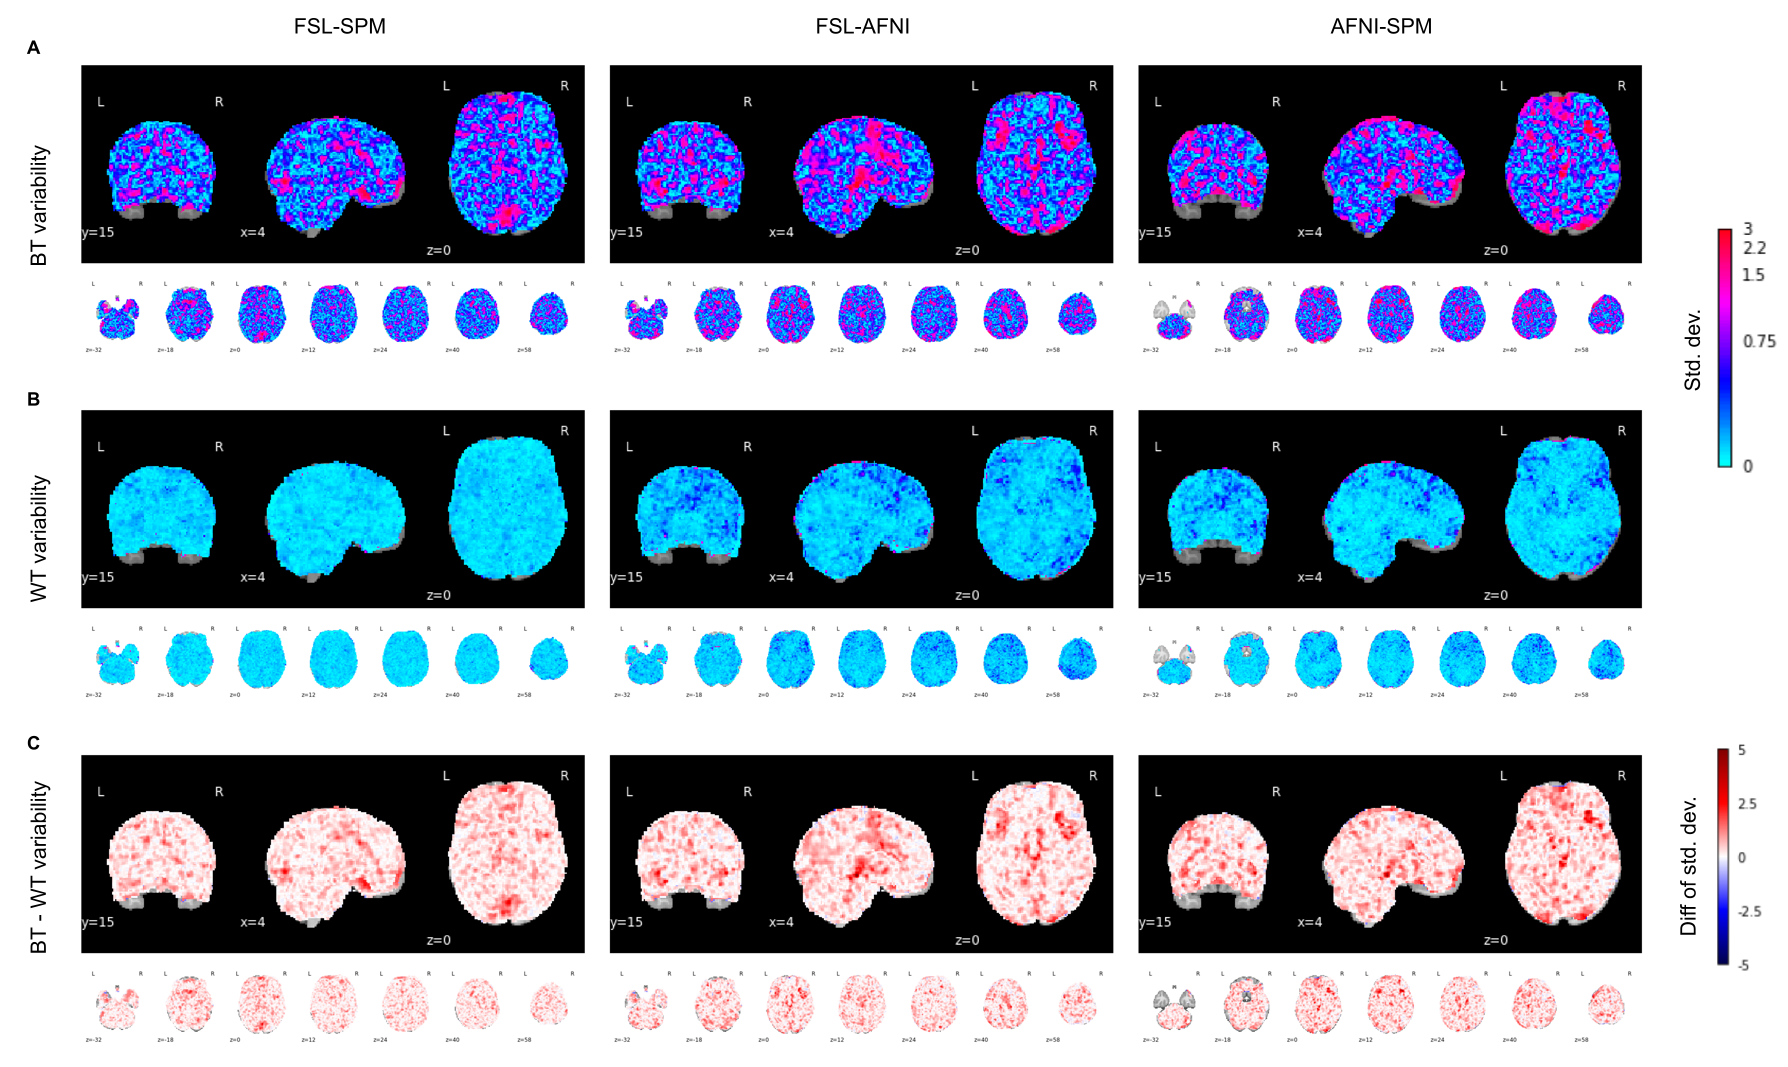
\includegraphics[width=\textwidth]{figures/std/gl-unthresh.png}
      %\caption{Standard deviation of thresholded t-statistics map on template surface}
    \caption{Unthresholded group-level variability computed between tools (\textbf{A}) and within tools (\textbf{B}), and difference between them (\textbf{C}).}
    \label{fig:unthresh-maps}
    \end{minipage}}
  \end{figure*}

  %%%%%%%%%% Corr. plot of tstats%%%%%%%%
  \begin{figure*}[ht]
    \fbox{\begin{minipage}{\dimexpr \textwidth-2\fboxsep-2\fboxrule}
      \begin{subfigure}[ht]{\textwidth}
        \centering
        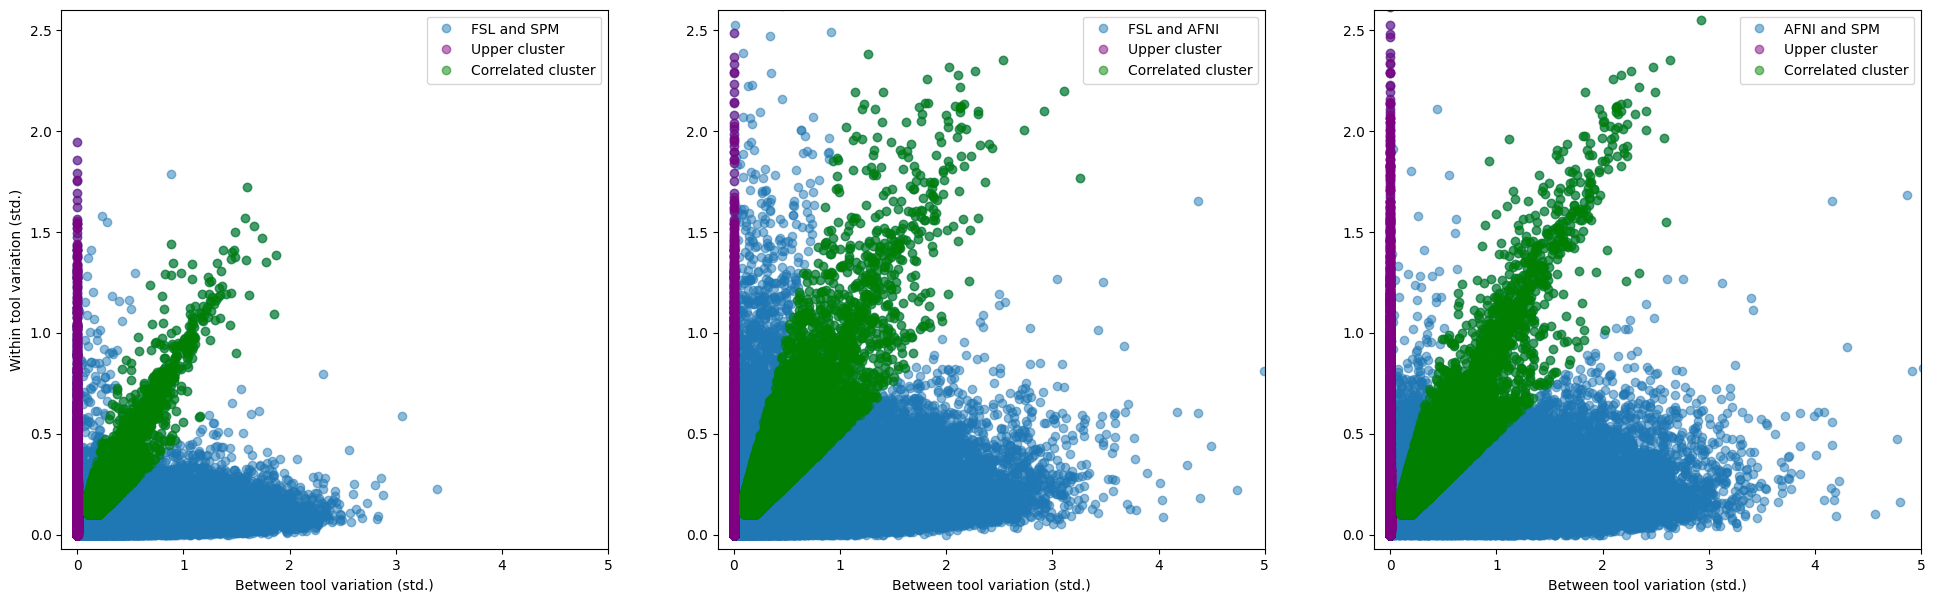
\includegraphics[width=\textwidth]{figures/std-corr-unthresh-plot.png}
        %\caption{Standard deviation of thresholded t-statistics map on template surface}
      \end{subfigure}
      \hfill
      \begin{subfigure}[ht]{\textwidth}
        \centering
        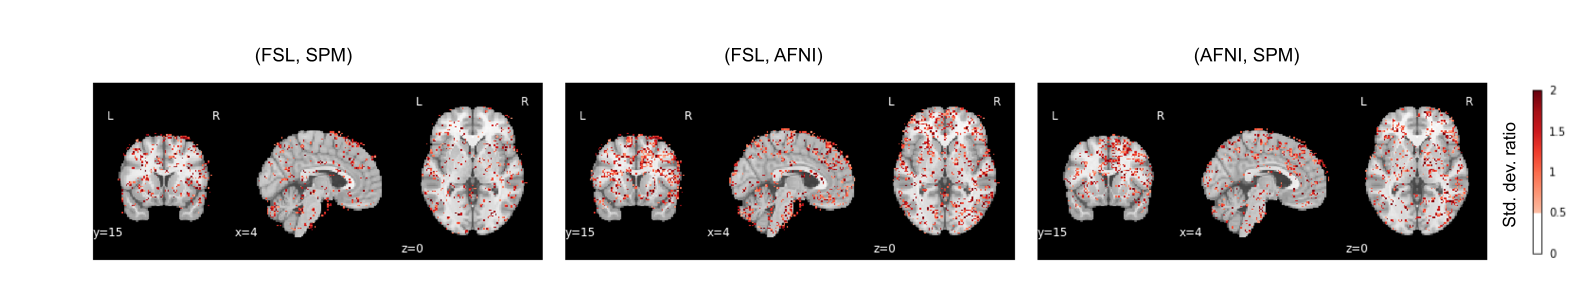
\includegraphics[width=\textwidth]{figures/std/correlated-unthresh.png}
        %\caption{Standard deviation of thresholded t-statistics map on template surface}
      \end{subfigure}
      \caption{
        Voxel-wise comparison of BT and WT variabilty. The bottom row shows 
        voxels where the BT/WT ratio is in (0.5, 2).}
    \label{fig:unthresh-correlation}
    \end{minipage}}
  \end{figure*}

  \subsection{Subject-level unthresholded maps}

  Summary statistics for subject-level unthresholded t-statistics maps are
  reported in Table~\ref{table:unthresh-maps-subjects}. As for group-level
  maps, BT variability was consistently larger than WT variability
  \tristan{report statistical tests}.

  Figure~\ref{fig:unthresh-maps-sbj} shows BT and WT variability for
  the subject with the highest WT variability among the 16 subjects. For
  this particular subject, WT variability approaches and even surpasses BT
  variability in some regions. This subject also revealed that WT
  variability mainly concentrated in some regions.

  %%%%%%%%%% Summary of statstics %%%%%%%%
\setlength{\tabcolsep}{5pt}
\begin{table}[h]
    \centering
    \begin{tabular}{cccc}
        \toprule
        \multirow{2}{*}{}& {} & \multicolumn{2}{c}{Unthresholded} \\
        \cmidrule{3-4} \\
        {} & {} & Mean & Std. dev. \\
        \midrule
        \rowcolor{lightgray}
        {Between Tools} & FSL vs. SPM        &  0.366       & 0.293     \\
        \rowcolor{lightgray}
        {(BT)} & FSL vs. AFNI                &  0.439       & 0.352     \\
        \rowcolor{lightgray}
        {} & AFNI vs. SPM                    &  0.491       & 0.381     \\
        {Within Tool} & FSL                  &  0.077       & 0.054     \\
        {(WT)}   & SPM                       &  0.048       & 0.037     \\
        {}   & AFNI                          &  0.108       & 0.131     \\
        \bottomrule
    \end{tabular} 
    \caption{Voxel-wise mean and standard deviation of BT and WT variability
    in subject-level t-statistics maps (averages on 16 subjects).}
    \label{table:unthresh-maps-subjects}
\end{table}


  %%%%%%%%%% Var. of Unthresh sbj05%%%%%%%%
\begin{figure*}[ht]
  \fbox{\begin{minipage}{\dimexpr \textwidth-2\fboxsep-2\fboxrule}
    \centering
    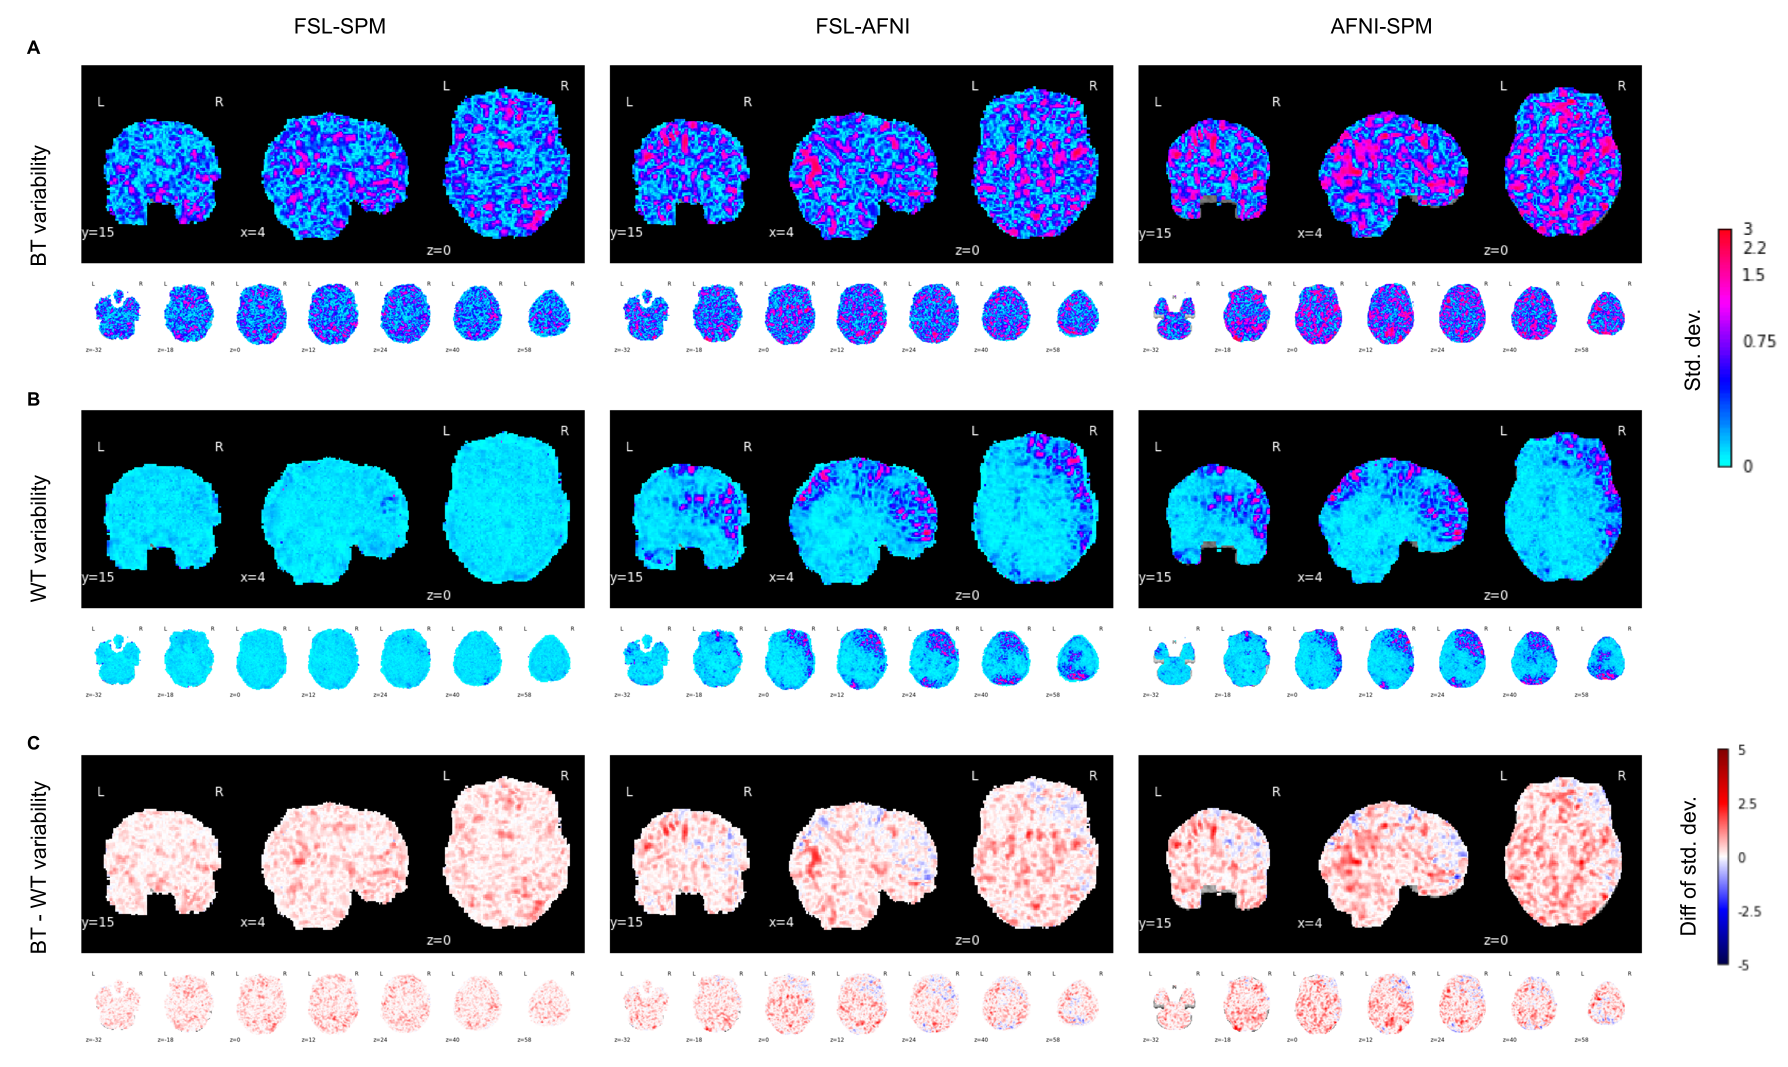
\includegraphics[width=\textwidth]{figures/std/sbj05-std.png}
    %\caption{Standard deviation of thresholded t-statistics map on template surface}
    \caption{For subject with highest WT variability, unthresholded subject-level variability computed between tools (\textbf{A}) and within tools (\textbf{B}), and difference between them (\textbf{C}).}
  \label{fig:unthresh-maps-sbj}
  \end{minipage}}
\end{figure*}

\begin{figure*}[ht]
  \fbox{\begin{minipage}{\dimexpr \textwidth-2\fboxsep-2\fboxrule}
    \begin{subfigure}[ht]{\textwidth}
      \centering
      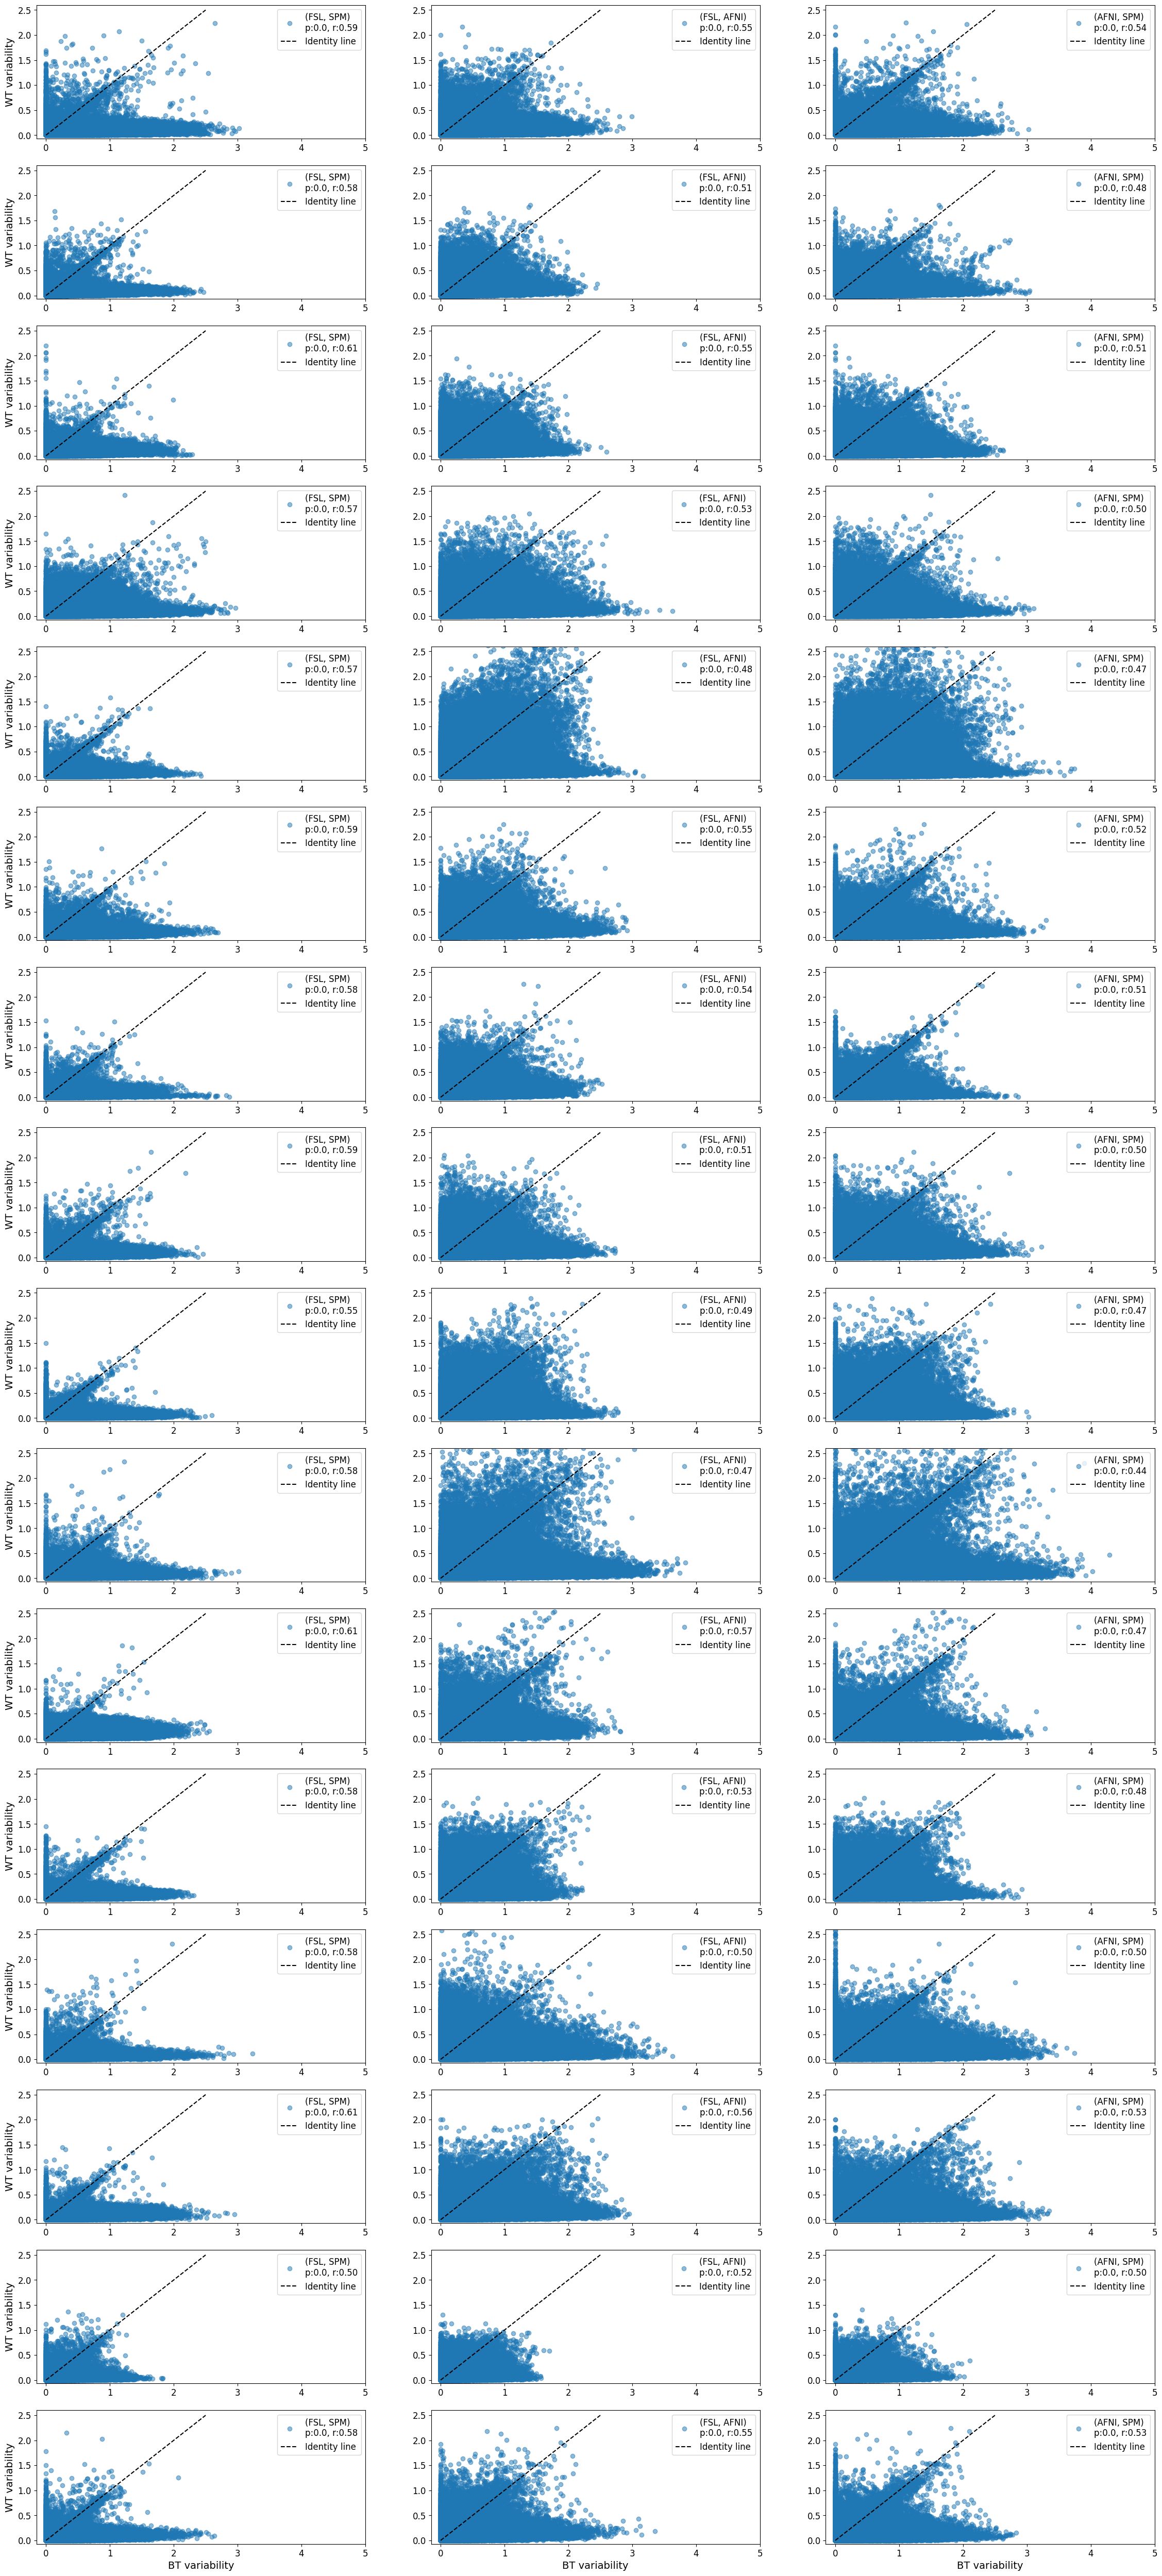
\includegraphics[width=.6\textwidth]{figures/sbj-std-corr-unthresh-plot.png}
      %\caption{Standard deviation of thresholded t-statistics map on template surface}
    \end{subfigure}
    \caption{
      Voxel-wise comparison of BT and WT variabilty subject by subject.}
  \label{fig:unthresh-correlation-allsbj}
  \end{minipage}}
\end{figure*}


\subsection{Group-level untresholded maps at different virtual precisions}

While the previous results were obtained at the virtual precision of 53~bits for double-precision values
and 24~bits for single-precision values, we also evaluated WT variability across different virtual precisions for FSL.
Figure~\ref{fig:across-precisions} shows the root-mean-square error (RMSE) between BT and WT variability maps.
The virtual precision of t=17 bits minimized the RMSE between BT and WT.
Figure~\ref{fig:gnp-mni} shows the corresponding BT and WT maps obtained at t=17 bits, showing 
that BT and WT reach comparable magnitudes in some regions.

  %%%%%%%%%% plot different precisions%%%%%%%%
  \begin{figure}[ht]
    \fbox{\begin{minipage}{\dimexpr \columnwidth-2\fboxsep-2\fboxrule}
        \centering
        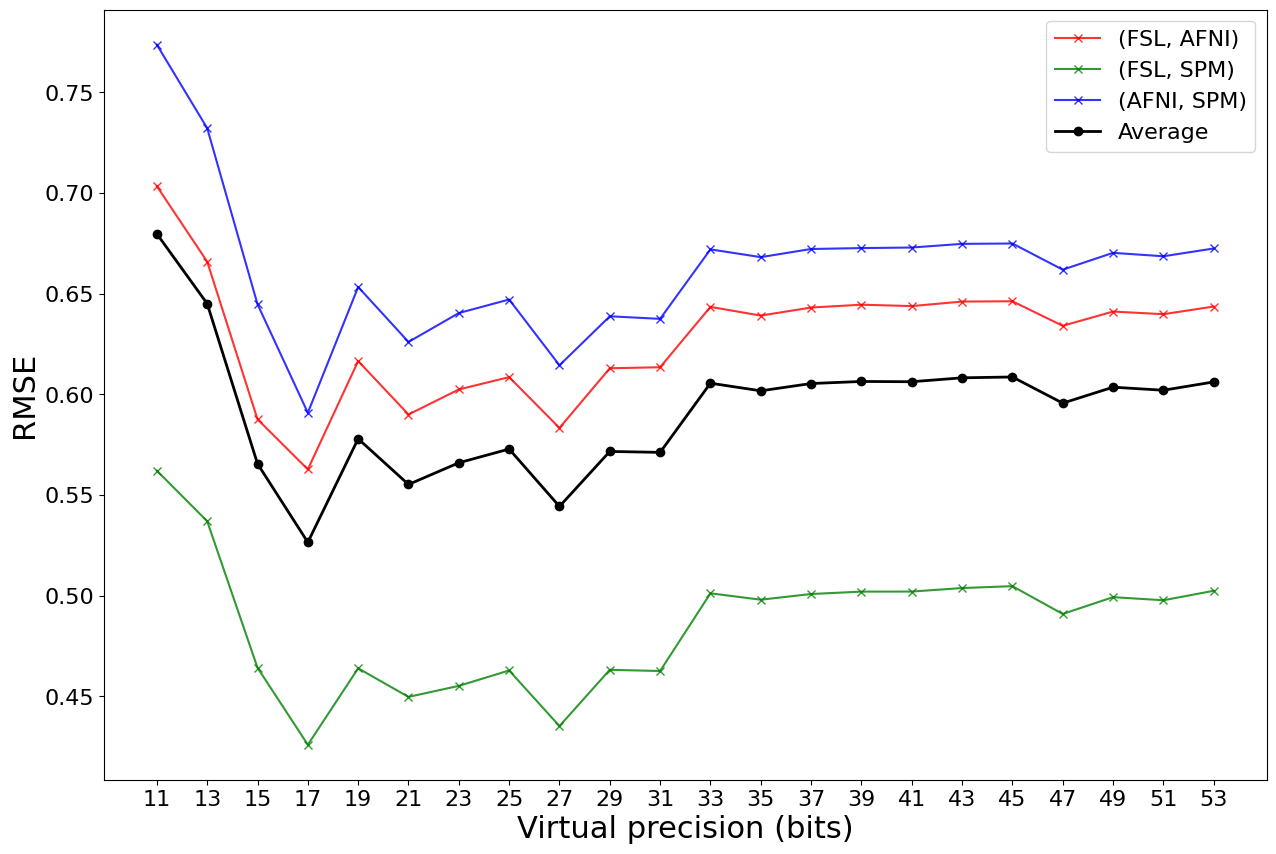
\includegraphics[width=\columnwidth]{figures/rmse-precisions.png}
        %\caption{Standard deviation of thresholded t-statistics map on template surface}
      \caption{Voxel-wise RMSE between BT and WT variability maps for different virtual precisions.}
    \label{fig:across-precisions}
    \end{minipage}}
  \end{figure}

  
  %%%%%%%%%% plot different precisions%%%%%%%%
  \begin{figure}[ht]
    \fbox{\begin{minipage}{\dimexpr \textwidth-2\fboxsep-2\fboxrule}
        \centering
        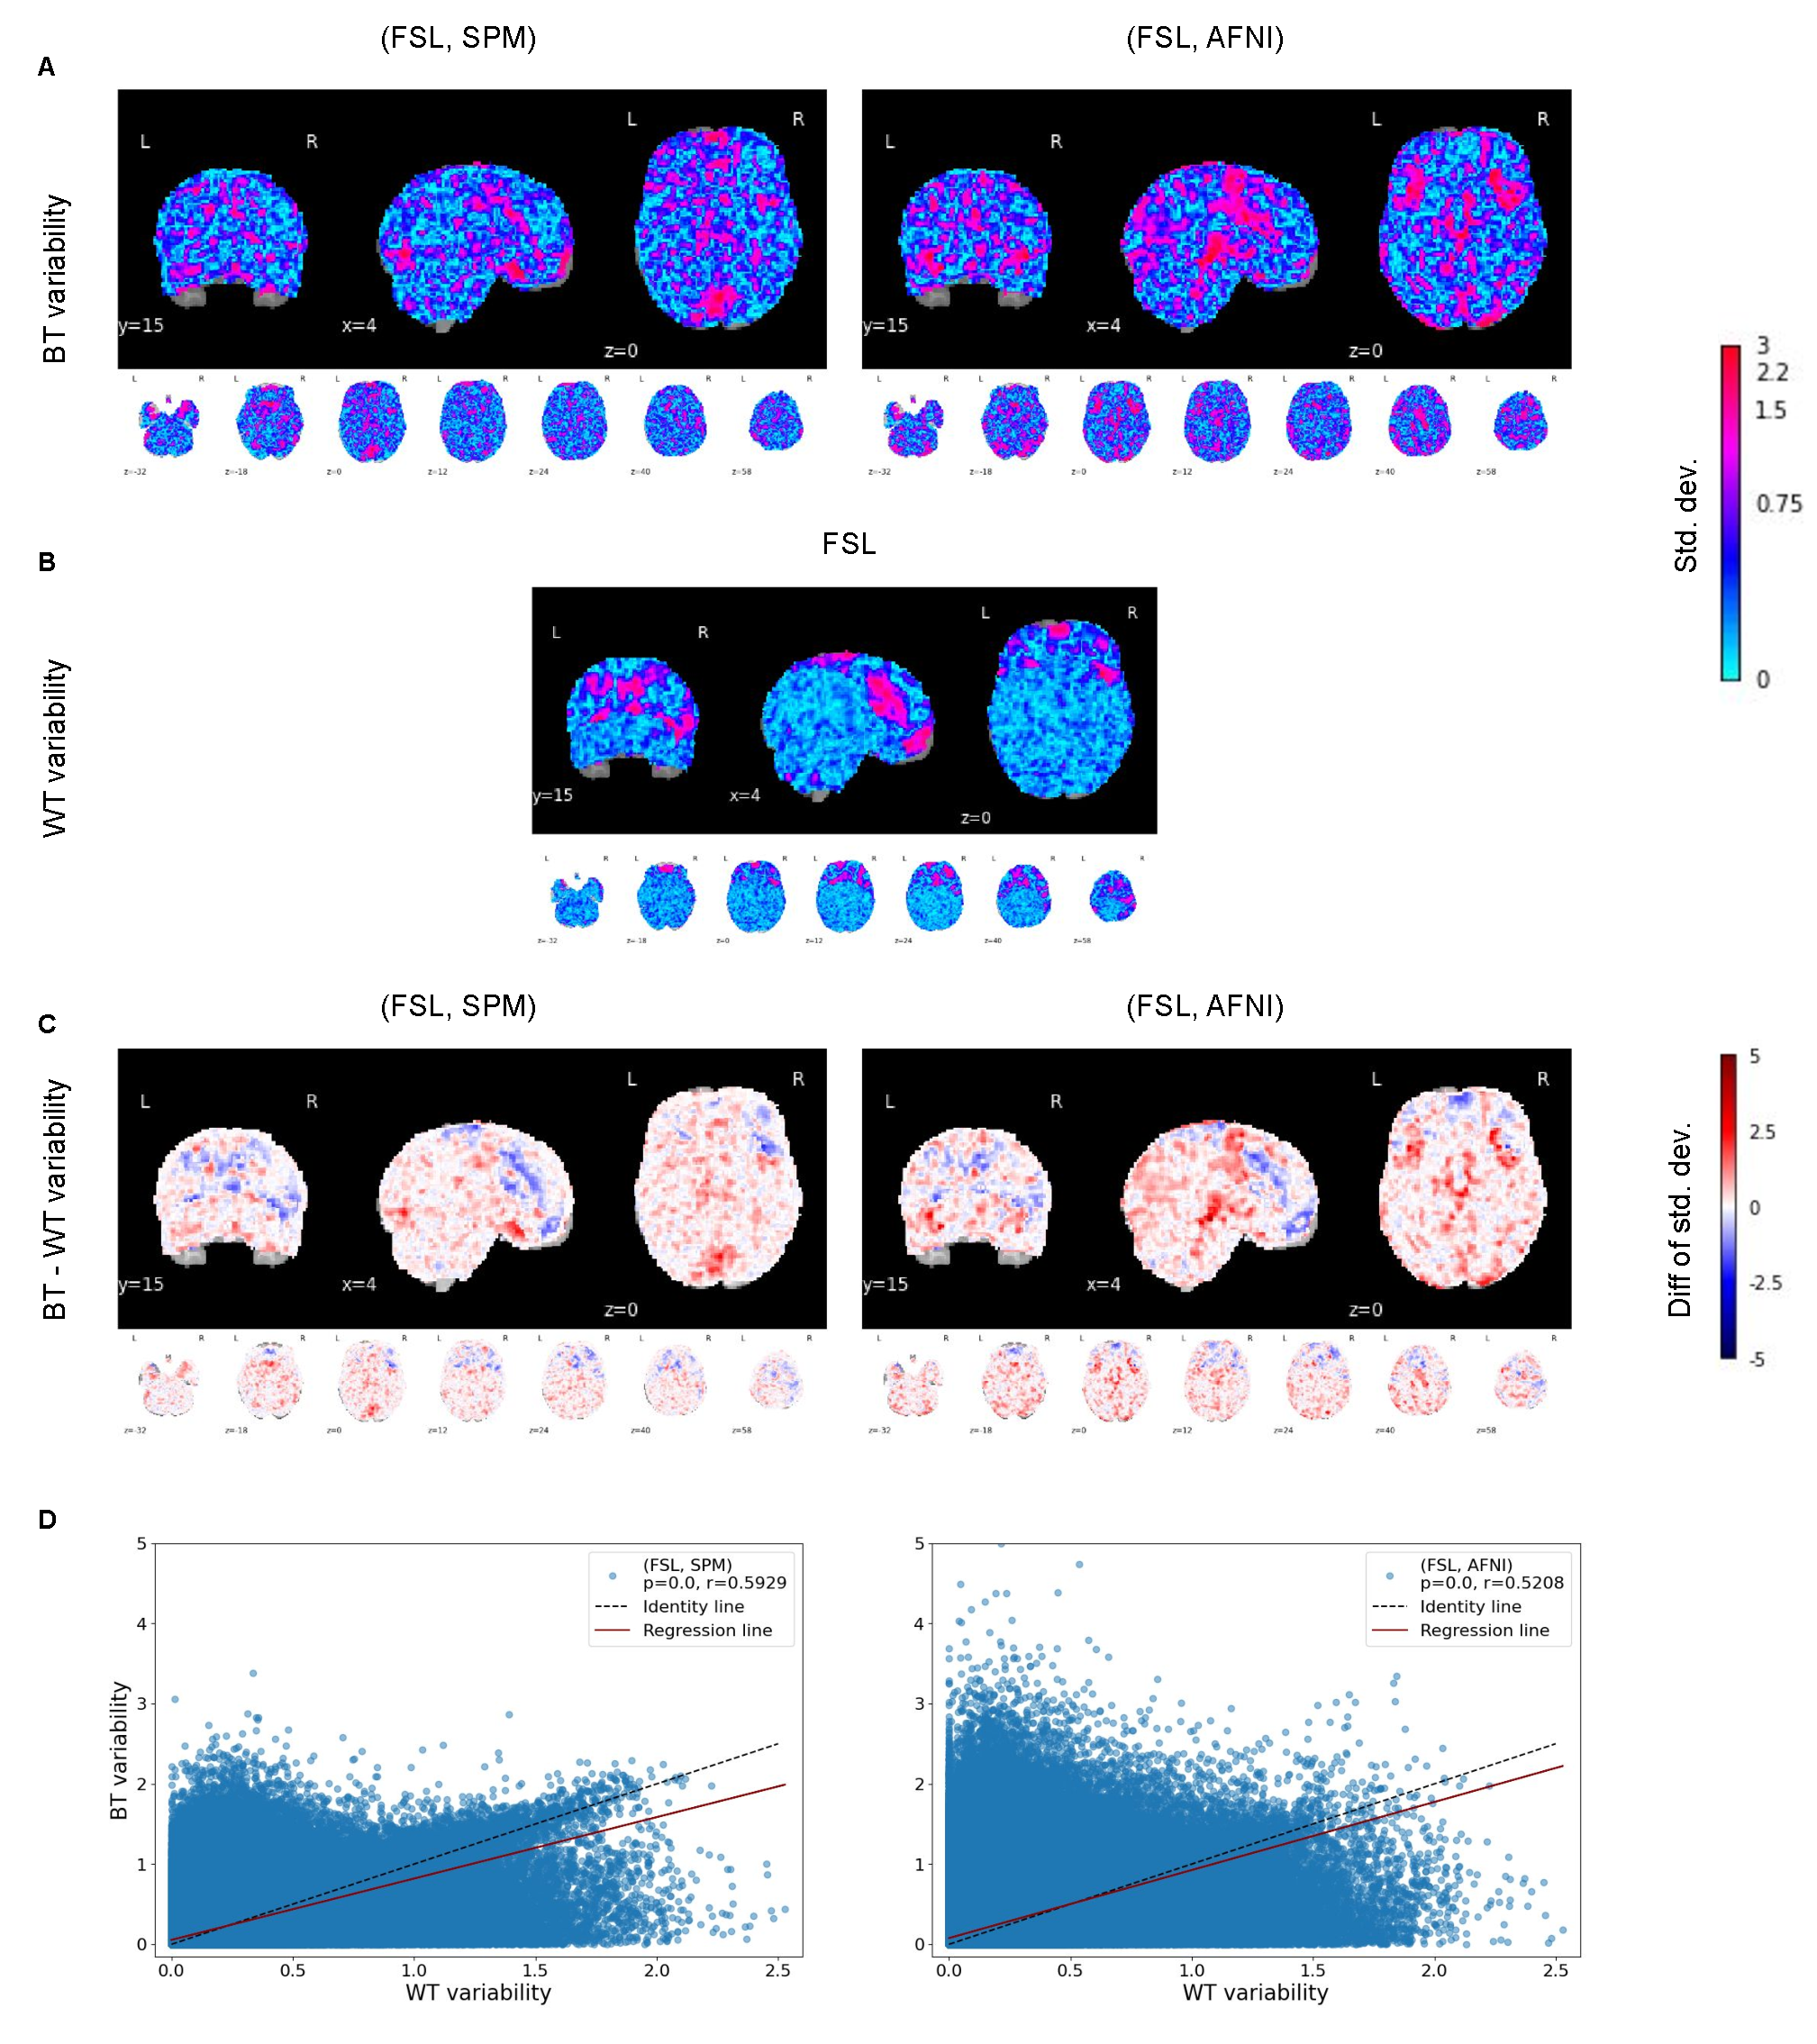
\includegraphics[width=.75\textwidth]{figures/bg_global_precision.pdf}
        %\caption{Standard deviation of thresholded t-statistics map on template surface}
        \caption{Unthresholded group t-statistics standard deviations computed between tools (\textbf{A}) and within tools (\textbf{B}), and difference between them (\textbf{C}).
        WT is computed at the virtual precision of t=17 bits.}
    \label{fig:gnp-mni}
    \end{minipage}}
  \end{figure}

  \begin{figure*}[ht]
    \fbox{\begin{minipage}{\dimexpr \textwidth-2\fboxsep-2\fboxrule}
      \begin{subfigure}[ht]{\textwidth}
        \centering
        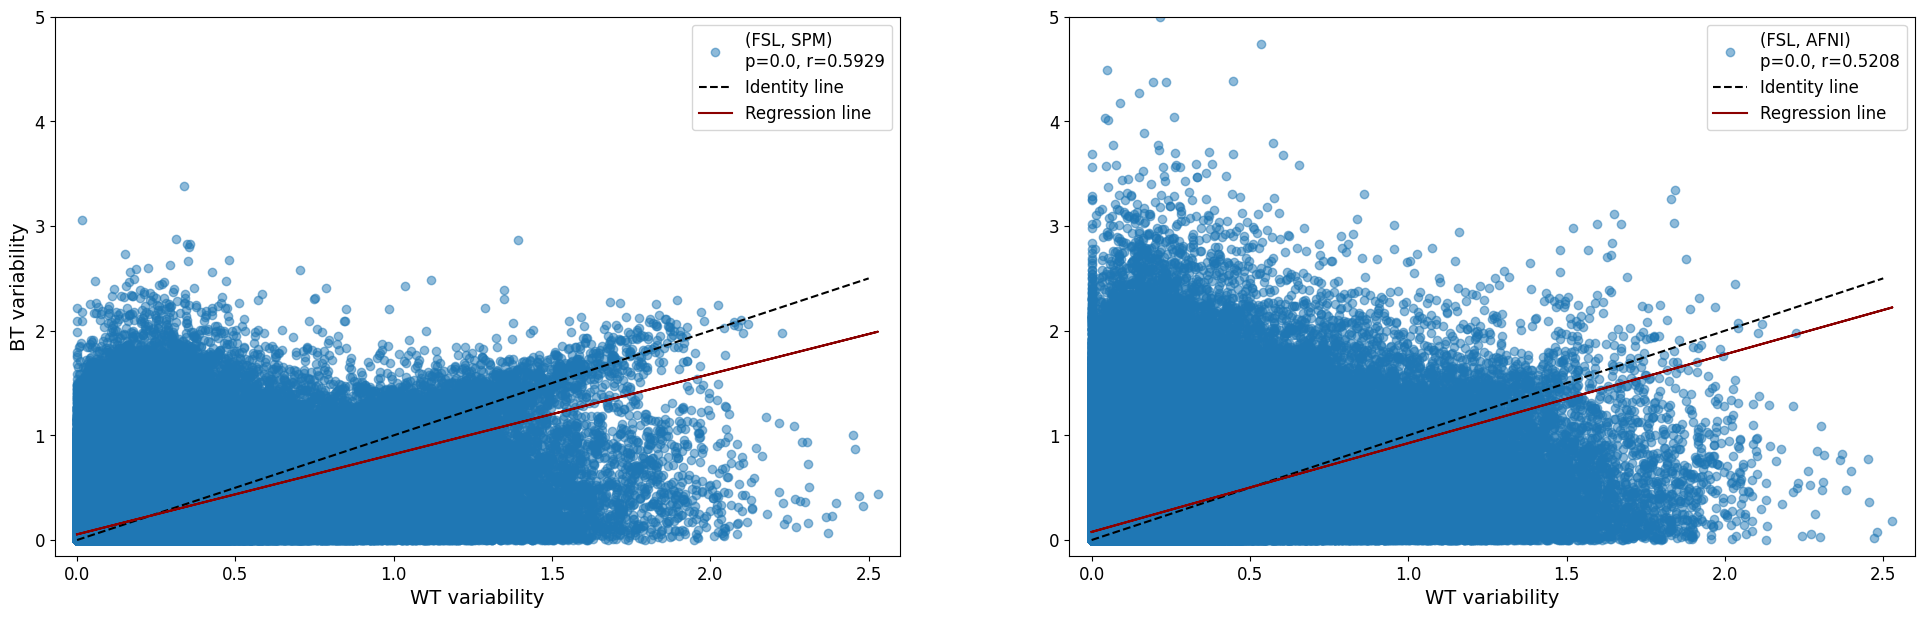
\includegraphics[width=\textwidth]{figures/std-corr-unthresh-vp17-plot.png}
        %\caption{Standard deviation of thresholded t-statistics map on template surface}
      \end{subfigure}
      \caption{
        Voxel-wise comparison of BT and WT variabilty. WT is computed with FSL at the virtual precision of t=17 bits.}
    \label{fig:unthresh-correlation-gvp}
    \end{minipage}}
  \end{figure*}


  \subsection{Group-level thresholded maps}

  Figure~\ref{fig:thresh-maps} compares BT and WT for thresholded group-level maps.
  While BT is consistently larger than WT, thresholding is an unstable operation 
  that results in comparable magnitudes for BT and WT within activation clusters where BT variability is low. 

  Figure~\ref{fig:cm-thresh} compares regional activation instability for BT and WT. The average ratio
  of unstable regions was 26\% for BT and 9.2\% for WT. Moreover, the average F1 score was 0.28. Therefore, regional 
  WT instability does not appear to be a 
  good predictor of BT instability.
  
  
  %%%%%%%%%% Var. of Thresh %%%%%%%%
  \begin{figure*}[ht]
      \fbox{\begin{minipage}{\dimexpr \textwidth-2\fboxsep-2\fboxrule}
        \centering
        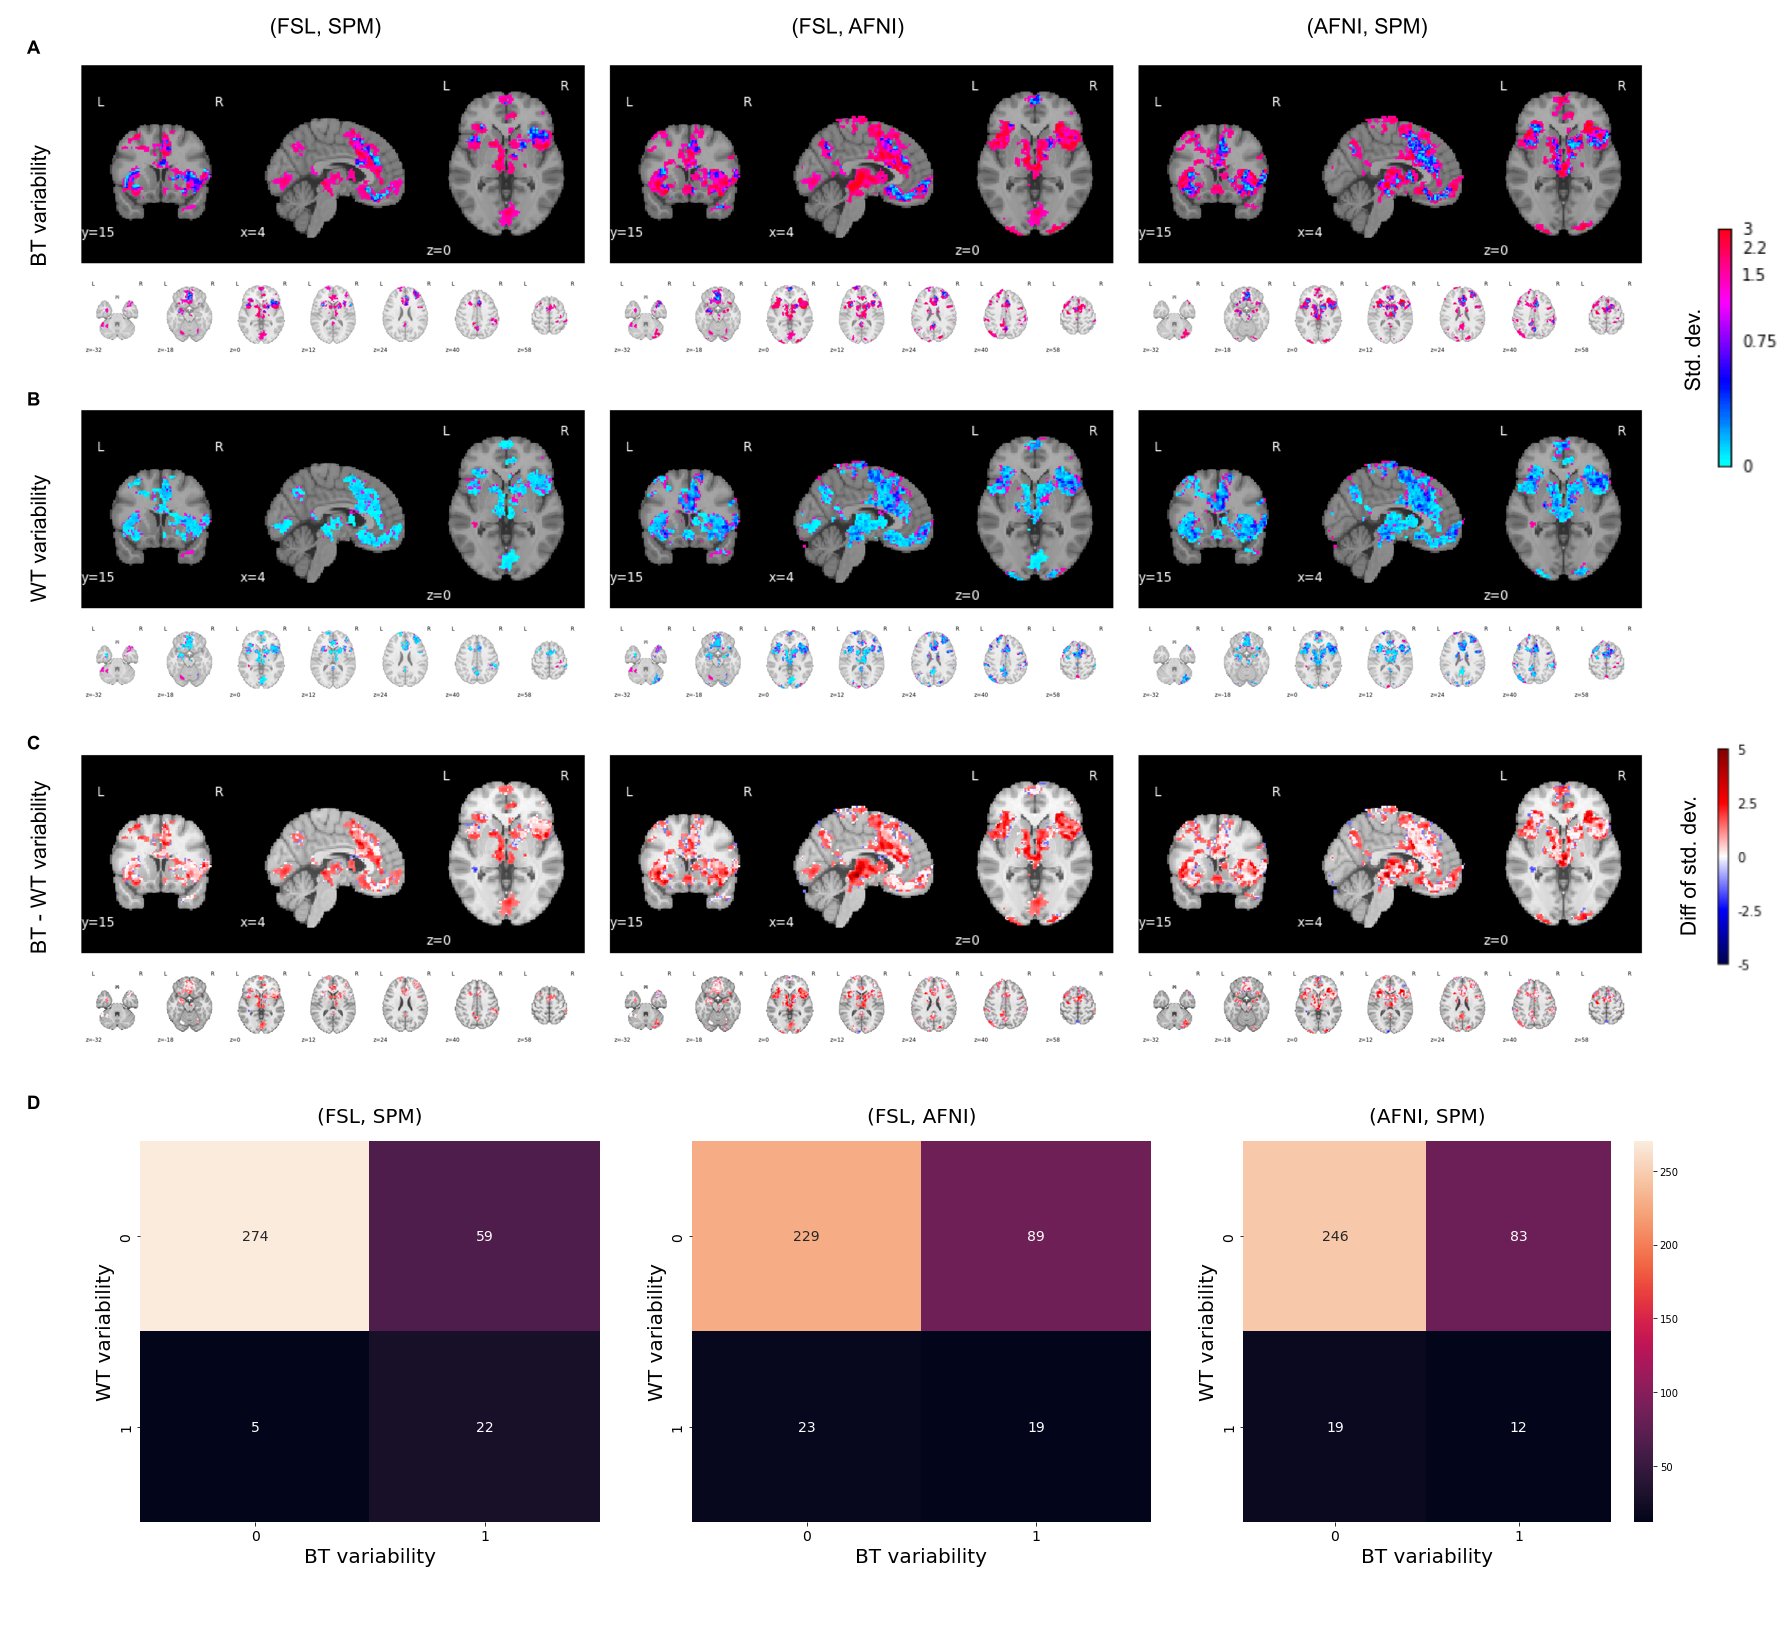
\includegraphics[width=\textwidth]{figures/std/gl-thresh.png}
      \caption{Thresholded group t-statistics standard deviation maps
      computed across tools (\textbf{A}) and Fuzzy Libmath samples
      (\textbf{B}).}
      \label{fig:thresh-maps}
      \end{minipage}}
    \end{figure*}
  
    % %%%%%%%%%% Dice plot of thresholded tstats%%%%%%%%
    \begin{figure*}[ht]
      \fbox{\begin{minipage}{\dimexpr \textwidth-2\fboxsep-2\fboxrule}
      \centering
      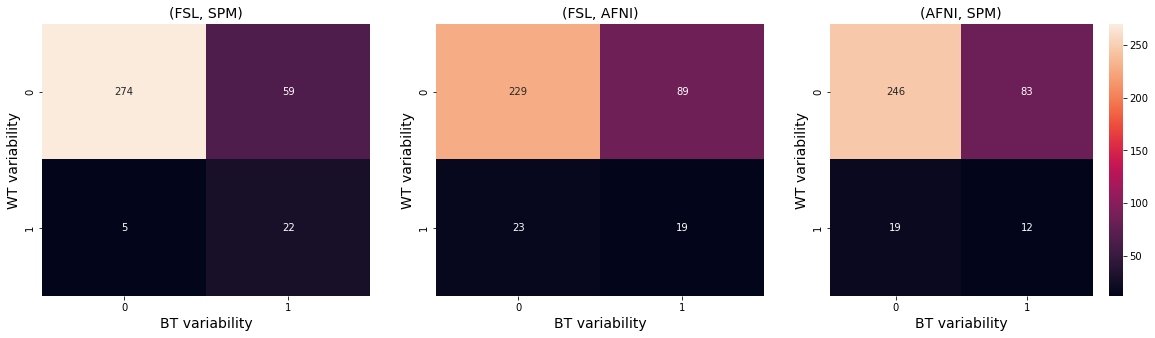
\includegraphics[width=\textwidth]{figures/dice_analysis-plot.png}
      \caption{Confusion matrices of activation instability
      in BT and WT among the 360 regions from the HCP-MMP1.0 parcellation.}
      \label{fig:cm-thresh}
    \end{minipage}}
    \end{figure*}

\section{Discussion}

In fMRI \emph{group analyses}, machine error remains an order of magnitude
smaller than between-tool variability. Group analyses have a regularization
effect toward numerical noise, which is expected to amplify as sample size
increases. Therefore, for fMRI studies with large sample sizes, machine
error can safely be neglected with respect to between-tool variability. The
recommendation made in~\cite{botvinik2020variability} to rely on ``multiverse" analyses where
multiple analysis tools are compared is therefore likely to successfully correct
for machine error in group studies.

However, machine error remains important in group analyses that are based
on a single tool, as is commonly the case in current fMRI studies. In
particular, in our study, the inherent instability of thresholding was
triggered by machine error in 9\% of 360 brain regions, which indicates
that machine error might have impacted neuroscientific conclusions related
to these regions. 

In \emph{subject analyses}, machine error and between-tool variabilty can
become comparable for some subjects in some regions. This observation is particularly
relevant to the development of fMRI-based biomarkers aiming at
individualized phenotype predictions. Machine error is expected to play
a non-negligible role in such analyses, even when predictions combine
results produced by multiple tools.

The observed regularization effect of group analyses toward numerical noise 
is consistent with observations made in~\cite{kiar2020numerical} from diffusion MRI where 
connectome graph statistics were found to be substantially unstable at the subject-level 
while group distributions remained consistent. 

\tristan{discuss larger numerical noise}

No association was found between
machine error and between-tool variability at the group or subject level,
which suggests that they can be investigated separately from each other.
Even though their effects can be of comparable magnitude, machine error and
between-tool variability are distinct and most likely involve different
root causes \tristan{revise this based on correlations}.

In conclusion, our results motivate further numerical stability
investigations in fMRI analysis pipelines. Pipeline-level analyses could be
conducted to identify specific components that contribute to numerical
variability, and if possible correct them accordingly. When instability is
inherent to the analysis, sampling results distributions through numerical
perturbations might improve stability, as explored in~\cite{kiar2021data}.
Finally, pipeline-specific statistical corrections might be envisaged to
account for numerical variability.




% No conclusion on which tool is more/less stable. 

\bibliographystyle{plain}
\bibliography{biblio}


\end{document}
\endinput
